\documentclass[10pt]{article}

\usepackage[paperheight=22.5 cm, paperwidth=17 cm, top=2 cm, bottom=2 cm, left=2.5 cm, right=1.5 cm]{geometry}
\usepackage[spanish,mexico]{babel}
\usepackage[utf8]{inputenc}
\usepackage{lscape} %Landscape mode
\usepackage[nottoc]{tocbibind} %Include bibliography in TOC

\usepackage[letter,cam,center]{crop}
\usepackage[labelfont=bf]{caption}

%\usepackage{graphicx} % OS X

\usepackage[pdftex]{graphicx} % Windows
\usepackage{epstopdf} % Windows

\renewcommand{\baselinestretch}{1.6} %double-spacing

\begin{document}

\thispagestyle{empty}
\tableofcontents
\newpage

\setcounter{page}{1}

\section{Descripción de las Base de Datos}
La Bolsa Mexicana de Valores proporcionó para este trabajo una base de datos con las posturas en todas las emisoras entre el 16 de noviembre de 2010 y el 18 de febrero de 2011. La base de datos se compone de dos tablas:

\begin{itemize}
  \item Posturas Iniciales
  \item Registro de Posturas
\end{itemize}

La tabla de registro tiene 25,491,702 renglones; mientras que la tabla de posturas iniciales tiene 275,005. En el registro se encuentran todas las posturas que reciben a lo largo del día. Las tablas tienen los siguientes campos:\\

\noindent
\begin{tabbing}
\textbf{id} \hspace{3cm} \= Número de identificación \hspace{1cm} \= \\
\\
\textbf{folio} \> Número asignado por la BMV a la postura\\
Según el reglamento de la BMV; las órdenes que, en su caso, tengan modificaciones,\\
perderán el folio de recepción que en un inicio les haya correspondido y se les asignará\\
uno nuevo. No perderán su folio aquellas órdenes que sean modificadas únicamente\\
para disminuir su volumen.\\
\\
\textbf{fecha\_vig/vigencia} \> Fecha de vigencia de la postura \\
\\
\textbf{casabolsa} \> Casa de Bolsa\\
\\
\textbf{tipo\_mov} \> Tipo de Movimiento\\
\underline{Posibles Valores} \\
CO \> Compra\\
VE \> Venta\\
MO \> Modificación\\
CA \> Cancelación\\
AH \> AH description\\
MH \> MH description\\
CH \> CH description\\
\\
\textbf{tipo\_op} \> Tipo de Operación\\
\underline{Posibles Valores} \\
CO \> Contado\\
PI \> Pico\\
HC \> Operación a Precio de Cierre\\
DC \> Operaciones al Precio de Cierre Modalidad Después del Cierre\\
OR \> Operaciones de Registro\\
OP \> Oferta Pública\\
SR \> Suscripción Recíproca\\
SA \> Sobre Asignación\\
\\
\textbf{tipo\_ord} \> Tipo de Orden\\
\underline{Posibles Valores} \\
LP \> Limitada\\
MC \> Mercado\\
MA \> Mejor Postura Limitada Activa\\
Aquella que sigue el mejor precio límite visible en su mismo sentido y su precio \\
buscará cerrar posturas en sentido contrario que se ubiquen dentro de su precio\\
de protección.\\
MP \> Mejor Postura Limitada Pasiva\\
Aquella que sigue el mejor precio límite visible en su mismo sentido. Aún y cuando\\
existan posturas en sentido contrario dentro de su precio de protección la postura\\
no buscará cerrarlas.\\
VO \> Postura Limitada con Volumen Oculto\\
LO \> Mejor Postura Limitada Activa con Volumen Oculto\\
HC \> Operación a Precio de Cierre\\
DC \> Operaciones al Precio de Cierre Modalidad Después del Cierre\\
PQ \> Paquete \\
\\
\textbf{tipo\_val} \> Tipo de Valor\\
\\
\textbf{emisora} \> Emisora\\
\\
\textbf{serie} \> Serie\\
\\
\textbf{precio} \> Precio\\
\\
\textbf{volumen} \> Volumen\\
\\
La tabla de posturas iniciales utiliza además estos campos:\\
\\
\textbf{fecha} \> Fecha\\
Este campo se utiliza para distinguir las órdenes que están activas al principio del\\
día e inicializar el libro de órdenes.\\
\\
\textbf{orig\_timestamp} \> Fecha original de la postura expresada como la cantidad de\\
\> milésimas de segundo transcurridas desde la medianoche del\\
\>1 de enero de 1970\\
\\
La tabla de registro utiliza estos campos:\\
\\
\textbf{timestamp} \> Fecha de la postura expresada como la cantidad de milésimas\\
\> de segundo transcurridas desde la medianoche del 1 de enero\\
\>de 1970\\
\\
\textbf{folio\_anterior} \> Folio Anterior\\
Se utiliza para localizar el folio de una postura que se va a modificar o cancelar.\\
\\
\textbf{fecha\_folio\_ant} \> Fecha de Folio Anterior\\
\end{tabbing}

\begin{landscape}

\begin{table}[htbp]\scriptsize
  \centering
  \caption{Posturas Iniciales}
 \setlength\tabcolsep{1.5pt}
    \begin{tabular}{rrrrrrrrrrrrrr}
   \textbf{ id}    & \textbf{fecha} & \textbf{orig\_timestamp} & \textbf{folio} & \textbf{fecha\_vig} & \textbf{tipo\_mov} & \textbf{casabolsa} & \textbf{tipo\_op} & \textbf{tipo\_ord} & \textbf{tipo\_val} & \textbf{emisora} & \textbf{serie} & \textbf{precio} & \textbf{volumen} \\
    247 & 24/11/2010 & 1290011934040 & 318480 & 10/12/2010 & CO    & 1277  & CO    & LP    & 1     & LAB   & B     & 25.95 & 2700 \\
    292 & 23/11/2010 & 1290189919100 & 368726 & 26/11/2010 & VE    & 1392  & CO    & LP    & 1     & CHDRAUI & B     & 39.8  & 100 \\
    519 & 23/12/2010 & 1292863358080 & 242642 & 24/12/2010 & VE    & 1277  & CO    & LP    & 1     & TELMEX & L     & 10.18 & 25000 \\
    651 & 27/01/2011 & 1295881813280 & 93317 & 28/01/2011 & VE    & 1664  & CO    & LP    & 1     & ASUR  & B     & 72    & 100 \\
    848 & 15/02/2011 & 1295539042060 & 268023 & 18/02/2011 & CO    & 1392  & CO    & LP    & 1     & INCARSO & B-1   & 12.01 & 1000 \\
    \ldots & \ldots & \ldots & \ldots & \ldots & \ldots & \ldots & \ldots & \ldots & \ldots & \ldots & \ldots & \ldots & \ldots \\
    \end{tabular}%
  \label{tab:posinicialesl}%
\end{table}%

\begin{table}[htbp]\scriptsize
  \centering
  \caption{ Registro de Posturas}
 \setlength\tabcolsep{1.5pt}
  \begin{tabular}{rrrrrrrrrrrrrrr}
   \textbf{ id}    & \textbf{timestamp} & \textbf{folio} & \textbf{vigencia} & \textbf{folio\_anterior} & \textbf{fecha\_folio\_ant} & \textbf{tipo\_mov} & \textbf{casa\_bolsa} & \textbf{tipo\_op} & \textbf{tipo\_ord} & \textbf{tipo\_val} & \textbf{emisora} & \textbf{serie} & \textbf{precio} & \textbf{volumen} \\
    48 & 1289916001700 & 19    &       & 0     &       & VE    & 1369  & CO    & LP    & 1     & MEXCHEM & *     & 39.6  & 800 \\
    329 & 1290785630710 & 124082 & 26/11/2010 & 0     &       & CO    & 1369  & CO    & LP    & 1     & AMX   & L     & 35.69 & 12000 \\
    519 & 1291907916550 & 16032 &       & 0     &       & AH    & 1305  & CO    & VO    & 1     & GFNORTE & O     & 58.1  & 1100 \\
    652 & 1296246310460 & 911020 &       & 0     &       & VE    & 1369  & PI    & MC    & 1     & ASUR  & B     & 64.05 & 76 \\
    998 & 1298062094720 & 566388 & 18/02/2011 & 566388 & 18/02/2011 & MO    & 1288  & CO    & MA    & 1     & BIMBO & A     & 97.51 & 300 \\
    \ldots & \ldots & \ldots & \ldots & \ldots & \ldots & \ldots & \ldots & \ldots & \ldots & \ldots & \ldots & \ldots & \ldots & \ldots \\
    \end{tabular}%
  \label{tab:regposturasl}%
\end{table}%

\end{landscape}

\begin{figure}[ht] \centering
\includegraphics[width=3.5in, height=3.5in]{plot.eps}
\caption{The normal density curve}
\label{normal}
\end{figure}

\newpage

\listoftables
\newpage

\nocite{*}

\bibliographystyle{apalike}
\bibliography{myrefs}

\end{document}